\documentclass[../catalog.tex]{subfiles}

\begin{document}

\subsubsection{Problem}

As has been widely documented within the database community
(\cite{leis2015good}, \cite{lohman2014query}), many complex queries
are highly sensitive to join ordering. We have discussed the
established heuristical approaches originating from
\cite{selinger1979access} in \ref{known-techniques} and hinted at
their various shortcomings.

There we concluded that cardinality estimation under the traditional
assumptions (uniformity, uncorrelated join predicates, overlapping key
domains, and full access to meaningful statistics) can not avoid
disastrous plans in all cases.

While improvements in data modeling, on-line gathering of index
statistics, and dynamic execution approaches such as Eddies provide
many interesting avenues of inquiry, we are interested in approaches
that make disastrous plans impossible.

The reasons for this are two-fold: first, and most importantly,
disastrous query plans violate all three of the desired properties
outlined in \ref{problem}. Second, from experiences with 3DF itself,
and other declarative systems such as the Prolog language, we know
that the mere \emph{possibility} of unpredictable, severe performance
degradations break the fundamental promise of the declarative
abstraction, and force users to reason defensively about the system
runtime.

We also covered recent advances in the area of worst-case optimal join
processing that introduce n-way join algorithms with improved
asymptotic complexity in some cases.

\subsubsection{Remedy}

\subsubsection{Evaluation}

First, we want to examine whether a worst-case optimal join strategy
does lead to more predictable latencies, \emph{irrespective of the
  clause order provided by the user}. For this we will consider the
triangle query \texttt{[?a :edge ?b] [?b :edge ?c] [?a :edge ?c]} on
the livejournal graph. The graph contains 68 million edges. We
introduce edges in node order, feeding them into a single
attribute. The i-th round of input is therefore that in which all
edges starting at node i are ingested. We use a single worker, running
on a single core of a 2.7 GHz Intel Core i5, with 16GB RAM available.

We run this setup for both strategies — consecutive binary joins
(\emph{JoinJoinJoin}) and worst-case optimal (\emph{Hector} — and for
three different input clause orders each, measuring completion time
for each round of inputs. The resulting latency distributions are
shown in figure \ref{fig:triangle-cdfs}.

\begin{figure}[h!]
  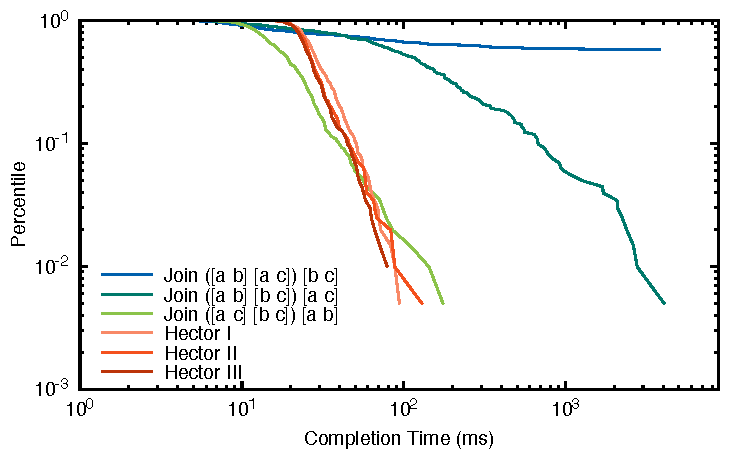
\includegraphics[width=1.0\linewidth]{results/triangles/out/all_cdfs}
  \caption{Triangle Query - Latency CCDFs}
  \label{fig:triangle-cdfs}
\end{figure}

As expected, we observe that performance of the JoinJoinJoin strategy
is highly sensitive to clause order. In particular, the first ordering
(\texttt{([a b] [a c]) [b c]}), runs out of memory at node 87, while
the third ordering (\texttt{([a c] [b c]) [a b]}) consistently
outperforms all of the tested strategies.

The worst-case optimal strategy performs consistently well for all
three input clause orderings and consistently outperforms the two
disastrous join orderings by one to many orders of magnitude. The best
performing JoinJoinJoin order can outperform Hector, but with a
similar long-tail and twice the maximum latency. [@TODO percentile
  table]

Figure \ref{fig:triangle-cdfs-extended} shows that these observations
remain valid when measuring thrice the number of rounds, as well as
when increasing the batch size to introduce one thousand nodes at a
time.

\begin{figure}[h!]
  \begin{subfigure}{.5\textwidth}
    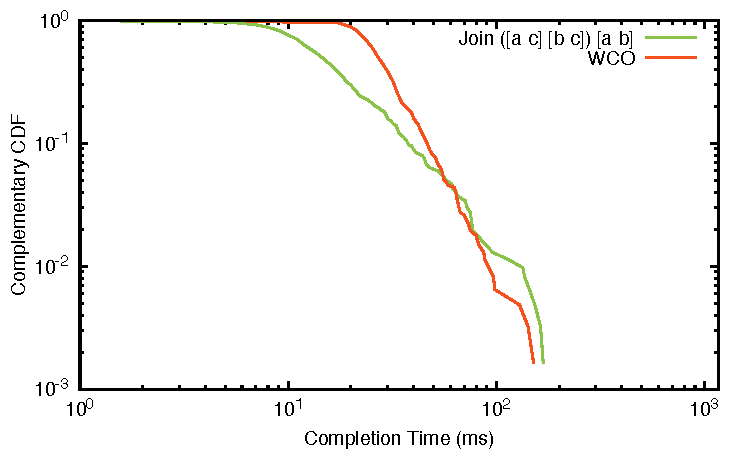
\includegraphics[width=1.0\linewidth]{results/triangles/out/extended_cdf}
    \caption{More Rounds}
  \end{subfigure}
  \begin{subfigure}{.5\textwidth}
    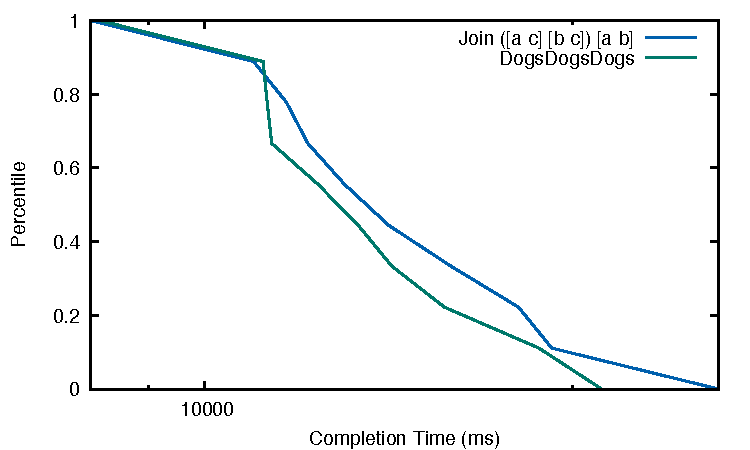
\includegraphics[width=1.0\linewidth]{results/triangles/out/batch_cdf}
    \caption{Batch Size 1000}
  \end{subfigure}

  \label{fig:triangle-cdfs-extended}
\end{figure}

\end{document}
